\documentclass{acm_proc_article-sp}

% UTF8 support
\usepackage[utf8x]{inputenc}
\usepackage[T1]{fontenc}

\usepackage{graphicx}
\graphicspath{{figs/}}
\usepackage{tikz}
\usetikzlibrary{shapes}

\usepackage{array}

\newcommand{\eg}{{\textit{e.g.~}}}
\newcommand{\etal}{{\textit{et al.~}}}
\newcommand{\ie}{{\textit{i.e.~}}}

\usepackage[draft, nomargin, footnote]{fixme}

\begin{document}

\title{A Model of the Dynamics of Anthropomorphism in Robotics}

\numberofauthors{3} 
\author{
\alignauthor
Séverin Lemaignan\\
    \affaddr{Computer-Human Interaction in Learning and Instruction}\\
    \affaddr{Ecole Polytechnique Fédérale de Lausanne (EPFL)}\\
    \affaddr{CH-1015 Lausanne, Switzerland}\\
    \email{severin.lemaignan@epfl.ch}
\alignauthor
Julia Fink\\
    \affaddr{Computer-Human Interaction in Learning and Instruction}\\
    \affaddr{Ecole Polytechnique Fédérale de Lausanne (EPFL)}\\
    \affaddr{CH-1015 Lausanne, Switzerland}\\
    \email{julia.fink@epfl.ch}
\alignauthor
Pierre Dillenbourg\\
    \affaddr{Computer-Human Interaction in Learning and Instruction}\\
    \affaddr{Ecole Polytechnique Fédérale de Lausanne (EPFL)}\\
    \affaddr{CH-1015 Lausanne, Switzerland}\\
    \email{pierre.dillenbourg@epfl.ch}
}
\date{30 July 1999}

\maketitle

\begin{abstract}

While anthropomorphism in robotics is a commonly discussed trait of HRI, it
paradoxically lacks formal grounds. Supported by extensive literature review
and long-term field studies, this article suggest to go beyond the traditional
perception of anthropomorphism as a static feature of a system: we propose to
understand anthropomorphism as a dynamic, non-monotonic and context-dependent
process, which evolves over time and accounts for special events such as the
so-called \textit{novelty effect}. To this end, we introduce a model of
anthropomorphism that analyzes the phenomenon along three interaction phases,
and we discuss cognitive and social interpretations that follow.

\end{abstract}

\terms{Experimentation, Human Factors}

\keywords{Anthropomorphism, Design, Human-Robot Interaction, Social Issues in Robotics, Acceptance of Robots}

\section{Anthropomorphism}
\label{sec:intro}

%DEFINITION OF ANTHROPOMORPHISM

The essence of anthropomorphism is the perception of human-like characteristics
in either real or imagined non-human agents. According to Epley \textit{et al.}
\cite{epley_when_2008}, these human-like characteristics may include physical
appearance, emotional states perceived to be uniquely human, or inner mental
states and motivations. Real or imagined non-human agents can be "anything that
acts -- or is believed to act -- with apparent independence, including
non-human animals, natural forces, religious agents, technological gadgets, or
mechanical devices". Such anthropomorphic representations are important
determinants of how a person perceives and in turn behaves towards these
agents, or how a person may behave in light of these agents
\cite{epley_when_2008}.

%ANTHROPOMORPHISM AS SUBJECT IN HCI AND HRI	
	
Phenomenons related to anthropomorphism -- along with questions such as "how
much human do we perceive in the non-human" or "how human-like do we treat
non-human artifacts" (and why?) -- have received remarkable attention in the
domains of Human-Computer Interaction (HCI) and Human-Robot Interaction (HRI):
the study of humans interacting with an artificial system / machine. Following
the \textit{Media Equation}, it has been described that people mindlessly react
socially to computers \cite{reeves_media_1996} and may even attribute human
(social) characteristics to their artificial counterpart. The phenomenon has
also been observed with virtual characters \fixme{cite [50, 100] in
rosenthal-von der Pütten (2013)}, and more recent studies investigated how
far people ascribe personality or intentions to artificial emobdied agents or
whether they show empathetic behavior toward robots
\cite{rosenthal-vonderputten_experimental_2013}. 

In this article we will use the term \emph{anthropomorphic effect} to denote
observable correlates of anthropomorphism. With these we include, amongst
others, verbal utterances (such as direct speech or the use of pronouns
"he/she"), (social) gestures (such as a hug, waving, deictic gestures) or
\fixme{anticipation of certain actions of an agent [what??]}.


\paragraph{Anthropomorphism in robotics}

Anthropomorphism is a commonly observed phenomenon in human-robot interaction.
Studies showed that there are people who directly talk to their robot (even if
it does not recognize speech), give it a name, greet it, wonder about its
intentions or actions
\cite{eyssel_anthropomorphic_2010,fink_anthropomorphic_2012,forlizzi_how_2007,fussell_how_2008,kiesler_anthropomorphic_2008}.
It has frequently been described that people ascribe intentions or emotions to
their domestic robot, such as to a Roomba vacuum-cleaning robot
\cite{krumm_my_2007,sung_robots_2009} or the AIBO robotic dog
\cite{friedman_hardware_2003}. People's tendency to anthropomorphize
technologies has besides been described earlier in human-computer interaction
and related to digital agents \cite{reeves_media_1996,
nass_anthropocentrism_1995}. 

Literature on anthropomorphism in robotics is quite diverse and one strives
hard to extract a coherent conclusion. One reason for this might be that
robotics is a multi-disciplinary field and researchers from very different
domains might integrate diverse or even contradictory understandings of the
phenomenon. Despite the fact that there is no commonly accepted definition of
anthropomorphism in robotics, and also the terminology is not clear, the terms
\textit{anthropomorphic} or \textit{human-like} are often used as if their
meanings were clear and agreed upon \cite{persson_anthropomorphism_2000}. Duffy
\cite{duffy_anthropomorphism_2002} even argues that the terms might be misused.
For instance, some researchers refer to \textit{"the robot's level of
anthropomorphism"} \cite{bartneck_is_2007}, whereas others argue that the
system or artifact itself does not "contain anthropomorphism" \textit{per se}
but only gives rise to the process of anthropomorphizing in a given user and
situation. Consequently, anthropomorphism emerges in the \textit{interaction}
between the technology and the user \cite{persson_anthropomorphism_2000}.

Paradoxically, anthropomorphism in the perception of non-human agents (such as
robots) is commonly observed but at the same time poorly understood
\cite{epley_seeing_2007}. What might also account for the rather poor (or
controversial) understanding of anthropomorphism in robotics, is the limited
reliability of some findings (or interpretations) from experiments
investigating anthropomorphism. Most of these experiments are conducted in
controlled lab-settings during short-term human-robot interactions. This
experimental setting (short term and laboratory context) can be critical when
studying a social phenomenon like anthropomorphism and possibly lead to
over-interpretations. 

To sum it up, while anthropomorphism in robotics is a commonly discussed and
studied trait of human-robot interaction, we think it is paradoxically an
overlooked research topic. The understanding of anthropomorphism in robotics
seems to not take into account the wide range of phenomena that it encompasses.
The traditional understanding of anthropomorphism in robotics to date considers
two main factors that account for the social phenomenon: the characteristics of
\textbf{1) the robot's design} (degree of human-likeness) and the psychological
determinants in \textbf{2) the human user} (see \cite{epley_seeing_2007}). It
has been shown that both these factors can facilitate or hinder
anthropomorphism. We propose to go beyond this traditional perception of
anthropomorphism as a static feature of HRI: Based on Persson \textit{et
al.}'s~\cite{persson_anthropomorphism_2000} argumentation that anthropomorphism
is a multi-layered phenomenon which arises in different levels, we suggest to
understand anthropomorphism as a \emph{dynamic}, \emph{context-dependent}
process. To this end, we apply Persson \textit{et al.}'s six levels on
anthropomorphism to HRI and introduce three \emph{interaction phases}. These
interaction phases of anthropomorphism reflect also the results of a long-term
study that we conducted in a real human environment and provide an account of
the so-called \textit{novelty effect}. We also draw attention to two new
determinants of anthropomorphism, namely, the context of use and the fact of
getting used to a system over time. We propose to add these two aspects as a
third factor, the characteristics of \textbf{3) the interaction} (time and
space), to the previous two factors of anthropomorphism (robot and user). 

\fxfatal{Add a 'paper overview'}
	
\section{A Model of the Dynamics of Anthropomorphism}
\label{sec:dynamics_model}


\begin{figure*}[htb]
\centering


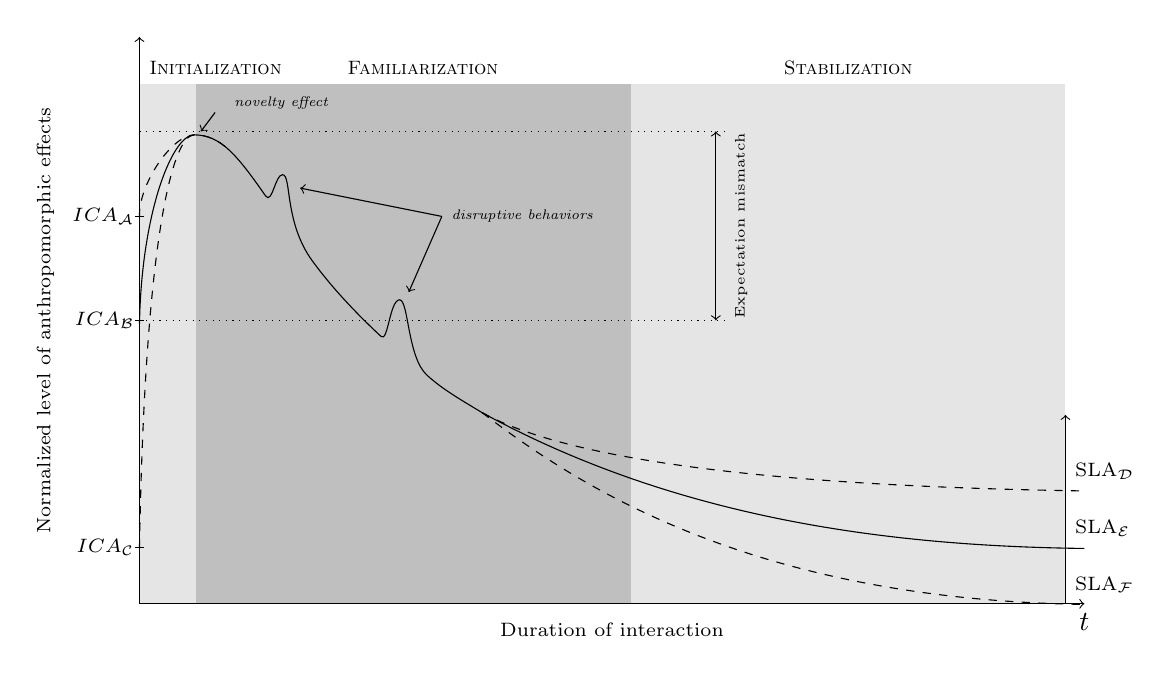
\begin{tikzpicture}[scale=1.2]

% background shading
\path[fill=gray!20] (0,0) rectangle (0.6,5.5);
\path[fill=gray!50] (0.6,0) rectangle (5.2,5.5);
\path[fill=gray!20] (5.2,0) rectangle (9.8,5.5);
\draw(0,5.5) node[anchor=south west] {\scriptsize \sc Initialization};
\draw(3,5.5) node[anchor=south] {\scriptsize \sc Familiarization};
\draw(7.5,5.5) node[anchor=south] {\scriptsize \sc Stabilization};
% horizontal axis
\draw[->] (0,0) -- (10,0) node[anchor=north] {$t$};
\draw(5,-0.1) node[anchor=north] {\scriptsize Duration of interaction};


% vertical axis
\draw[->] (0,0) -- (0,6) node[anchor=east] {};
\draw(-0.8,3) node[rotate=90,anchor=south] {\scriptsize Normalized level of anthropomorphic effects};

\draw (-0.05, 3) -- (0.05, 3) node[anchor=east] {\scriptsize $\text{ICA}_{\mathcal B}$};
\draw (-0.05, 4.1) -- (0.05, 4.1) node[anchor=east] {\scriptsize $\text{ICA}_{\mathcal A}$};
\draw (-0.05, 0.6) -- (0.05, 0.6) node[anchor=east] {\scriptsize $\text{ICA}_{\mathcal C}$};

% vertical axis - end
\draw[->] (9.8,0) -- (9.8,2) node[anchor=east] {};
\draw (9.8, 0.8) node[anchor=west] {\scriptsize SLA$_\mathcal{E}$};
\draw (9.8, 1.4) node[anchor=west] {\scriptsize SLA$_\mathcal{D}$};
\draw (9.8, .2) node[anchor=west] {\scriptsize SLA$_\mathcal{F}$};


\draw[<-] (0.65,5) -- (0.8,5.2) node[anchor=east] {};
\draw (0.9,5.3) node[anchor=west] {\tiny \it novelty effect};


\draw[dotted] (0, 5) -- (6.2,5);
\draw[dotted] (0, 3) -- (6.2,3);
\draw[<->] (6.1,3) -- (6.1,5) node[anchor=east] {};
\draw (6.2,4) node[rotate=90, anchor=north] {\tiny Expectation mismatch};

\draw[<-] (1.7,4.4) -- (3.2,4.1) node[anchor=east] {};
\draw[<-] (2.85,3.3) -- (3.2,4.1) node[anchor=east] {};
\draw (3.2,4.1) node[anchor=west] {\tiny \it disruptive behaviors};
%%%%%
%% CURVES
%%%%
\begin{scope}[yscale=-1,shift={(-0.125,-0.4)}]

% output of inkscape2tikz
\path[draw=black]
    (0.1250,-2.5620) .. controls (0.1451,-3.7193) and (0.4645,-4.5602) ..
    (0.7044,-4.5633) .. controls (0.8413,-4.5633) and (0.9599,-4.5104) ..
    (1.0794,-4.3971) .. controls (1.1989,-4.2841) and (1.3191,-4.1185) ..
    (1.4588,-3.9181) .. controls (1.5287,-3.8183) and (1.5610,-4.1413) ..
    (1.6381,-4.1420) .. controls (1.7378,-4.1420) and (1.6515,-3.6434) ..
    (1.9554,-3.2280) .. controls (2.1466,-2.9667) and (2.3889,-2.7023) ..
    (2.6819,-2.4292) .. controls (2.7551,-2.3607) and (2.7727,-2.8119) ..
    (2.8771,-2.8180) .. controls (2.9742,-2.8180) and (2.9594,-2.2108) ..
    (3.1665,-2.0209) .. controls (3.3340,-1.8673) and (3.5379,-1.7527) ..
    (3.7508,-1.6236) .. controls (5.8366,-0.4852) and (8.0977,-0.2106) ..
    (10.1250,-0.1860);
\path[draw=black, dashed]
    (0.1250,-3.6924) .. controls (0.1103,-4.0298) and (0.4645,-4.5602) .. 
    (0.7044,-4.5633)
    (3.7508,-1.6236) .. controls (4.9579,-0.9555) and (8.1358,-0.8261) .. 
    (10.1250,-0.7946);
\path[draw=black,dashed]
    (0.1250,-0.1953) .. controls (0.1804,-3.3871) and (0.4645,-4.5602) .. 
    (0.7044,-4.5633) .. controls (0.8413,-4.5633) and (0.9599,-4.5104) .. 
    (1.0794,-4.3971)
    (3.7508,-1.6236) .. controls (4.7654,-0.8505) and (6.5955,0.3538) .. 
    (10.1250,0.4062);

\end{scope}

\end{tikzpicture}

\caption{Dynamics of anthropomorphism. We distinguish three main phases:
\emph{initialization}, \emph{familiarization} and \emph{stabilization},
preceded by a \emph{pre-interaction} phase. In the pre-interaction phase,
users build an \emph{initial capital of anthropomorphism} (ICA). Once the
interaction starts, the level of anthropomorphism increases due to the
\emph{novelty effect}, and then decreases to reach a \emph{stabilized level
of anthropomorphism} (SLA).  During the interaction, unpredicted behaviors
of the robot (\emph{disruptive behaviors}) may lead to local increase of the
level of anthropomorphism.}

\label{fig:dynamics}
\end{figure*}


The underlying process in anthropomorphism is understood as reasoning about and
perceiving something non-human, and unknown or unfamiliar based on one's
representation of the familiar and well-known concept of being human (or
one-self). The basic operations underlying inductive inference are the
acquisition of knowledge, the activation or elicitation of knowledge, and the
application of activated knowledge at the time of the judgment
\cite{epley_when_2008}. According to Epley \textit{et al.}, the application
includes attempts to correct, adjust, or integrate less accessible information
into a more automatically activated default representation. This process can be
seen as a process of correction, and thus, it is often insufficient leaving
final judgments biased in the direction of the initially activated
representation. As a person's knowledge base changes / evolves constantly with
newly acquired things, or growing experiences with a robot, etc., it is likely
that the "need to anthropomorphize" a robot decreases over time. First, because
of the evolved knowledge about it, and second because one has familiarized
oneself with it.  Consequently, the robot should become more predictable and
more familiar to the human user and inferences about it can be made based on
the acquired knowledge.

\subsection{Model of anthropomorphism over time}
\label{sec:modelintro}

So far, the HRI community has not much investigated how anthropomorphism in
human-robot interactions evolves over time (during the process of
\emph{adopting} a robot, for instance): we propose to go beyond the traditional
perception of anthropomorphism in robotics as a static feature that once
observed during a short-term interaction reflects a sustaining social effect.
Based on an extensive literature review previously
published~\cite{fink_anthropomorphism_2012} and \fixme{our own work}
\fxfatal{Summarize these findings in a specific section!}, we believe that
anthropomorphic effects in HRI are not always the same but evolve over time,
along with growing interaction and experience with the robot, similar to how
relationships among people evolve over time \fixme{(cite Hinde, 1988)}. In
fact, Kanda \textit{et al.} \cite{kanda_interactive_2004} also hypothesized
that people's attitude toward technological artifacts and their relationship
with them would evolve over time, and they were among the first who described
\textit{novelty effects} during a long-term study with an interactive robot in
a school.

The model of anthropomorphism we propose (Figure~\ref{fig:dynamics}) represents
how the level of anthropomorphic effects (\ie observable manifestations of
anthropomorphism, as defined in section~\ref{sec:intro}) evolves over a
long-term human-robot interaction. By long-term interaction, we mean direct
(non-mediated), repeated interaction with the same robot, over at least several
days. The nature of the interaction (goal-directed, entertainment, etc.) may
however vary.

Anthropomorphism is quantified by a \emph{normalized level of anthropomorphic
effects}: because anthropomorphic effects are not quantified on an absolute
scale, we present them as a normalized value, that spans from a minimum (no
anthropomorphic effects) to a maximum (corresponding to the novelty effect peak
on Figure~\ref{fig:dynamics}). The actual maximum value of anthropomorphic
effects depends on each unique combinations of human, robot and several other
factors we introduce below, and thus varies. The general \emph{shape} of the
model remains however the same and depicts the evolution of anthropomorphism over
time, \ie the general dynamics of anthropomorphism.

The model takes into account the duration of the interaction, the nature of the
interaction, as well as acquired experience and familiarization mechanisms. We
also formally introduce a so-called \emph{novelty effect} that
models the first phase of human-robot interaction, during which a specific
increase of anthropomorphic interactions is observed.

\subsection{Three phases}
\label{sec:phases}

We distinguish three main phases that describe the evolution of the
anthropomorphic effects in a long-term human-robot interaction. They are
depicted in different shades on Figure~\ref{fig:dynamics}.

\subsubsection{Initialization Phase}
\label{sec:initialization}

During this short phase (from a couple
of seconds to a couple of hours), we observe an increased level of
anthropomorphism, from an \emph{initial capital of anthropomorphism}
(detailed in the next section) to a peak of anthropomorphic manifestations
that corresponds to the maximum of the \emph{novelty effect}.

\paragraph{Initial Capital of Anthropomorphism}
\label{sec:ica}

A robot has an initial potential of being anthropomorphized. It has been shown
that some \textit{people} anthropomorphism more than others, some
\textit{situations} induce anthropomorphism more than others, that
\textit{children} tend to anthropomorphize more than adults, and some
\textit{cultures} are notorious for their anthropomorphic religions and
worldviews \cite{epley_when_2008}. Our model of anthropomorphism takes these
determinants into account and initializes the level of anthropomorphic
interactions between a human and a robot to a value that we call
\textit{initial capital of anthropomorphism} (ICA on
Figure~\ref{fig:dynamics}). The ICA describes the first (real or imagined)
contact to a robot. In this stage of "pre-interaction", people form initial
expectations toward the robot and imagine how they will use / interact with it.

We build the ICA on three main factors that \textit{a priori} determine the
potential that a robot will be anthropomorphized:

\begin{enumerate}

    \item \emph{Human-centered factor}: The \textbf{personality} and individual
        traits of the human user: Psychological characteristics / determinants
        that influence a person's tendency to anthropomorphize
        artifacts~\cite{epley_seeing_2007}. Other individual traits and
        demographic aspects are comprised (\eg age, gender, cultural
        background, professional background).
	
    \item \emph{Robot-centered factor}: The robot's \textbf{design} and how it
        appears to the human user. Characteristics of the robot's form,
        behavior, and interaction modalities (anthropomorphic
        design)~\cite{fong_survey_2003}.
	
    \item \emph{Situation-centered factor}: The real or imagined
        \textbf{purpose} of the robot, including the situational context in
        which it is used. The task context and role in which the robot is used
        / experienced (environmental context)~\cite{joosse_what_2013}.

\end{enumerate}	

By \textbf{purpose} we suggest that the real or imagined context in which a
robot is used and the interaction that it brings along, impacts how far the
robot will be attributed human-like characteristics. We draw on findings such
as presented in Joosse \textit{et al.}\fxfatal{reference?}. The authors showed
that when the same robot (NAO) is used in a different task context (cleaning
task \textit{vs.} tour guide), this influences the perception of the
"personality" of the robot. In general, we think that a robot which is imagined
to be used in a social, entertaining or playful context leads to a higher ICA
than a robot which is used for a serious task (security, rescue, etc.). This
idea receives support from \fixme{XX (Kiesler / Goetz?)} work that revealed
that people prefer a serious robot for serious tasks and a less serious robot
for more playful tasks \fixme{REF}. Also, we suggest that the environmental
context in which people experience and interact with the robot impacts the ICA.
When several people who might be friends interact simultaneously with the robot
this might lead to an increased ICA \fixme{study: people are more emotional
when watching TV in company than when watching TV on their own}.

\paragraph{The Novelty Effect}
\label{sec:noveltyeffect}

\subsubsection{Familiarization Phase}
\label{sec:familiarization}

The second phase, \emph{familiarization}, lasts longer (up to several days) and
models the process of the human getting acquainted to the robot: by observation
and interaction, the human builds a model of the robot's behavior that allows
him/her to predict the robot's actions. We observe a decrease of
anthropomorphic effects during this phase, that we explain by the acquired
ability to predict the behavior of the robot: the initial apparent behavioral
complexity vanishes, and the robot is considered more and more as a tool.

\paragraph{Disruptive behaviors}

By \emph{disruptive behaviors}, we mean any behavior exhibited by the robot
that is unexpected by the user: for instance, a robot may usually follow always
the same route to go to two different places in a house, and suddenly change
the route. The actual underlying reason may span from a bug to the detection of
a new possible obstacle, but as long as this reason is not immediately
intelligible to the user, the behavior counts as \emph{disruptive}.

Our model represents \emph{disruptive behaviors} as local increases of
anthropomorphic effects in the familiarization phase (and at a lesser extend,
in the stabilization phase) (Figure~\ref{fig:dynamics}): because such behaviors
are unexpected, a human observer interprets them as the result of a richer
deliberative process.

This is however to be modulated depending on the real and percieved reasons of
the unexpected behavior. It may increase if the user perceives (rightfully or
not) a form of intentionality, as well as decrease if the unexpected behavior
is perceived as a failure.

\subsubsection{Stabilization Phase}
\label{sec:stabilization}

The last phase is the \emph{stabilization} phase. The level of anthropomorphic
effects tends to stabilize over a longer time, to reach a \emph{stabilized
level of anthropomorphism} (SLA).

If, after the familiarization phase, no anthropomorphic effects are observed
anymore, the \emph{Stabilized Level of Anthropomorphism} is zero. This can
be interpreted as the user interacting with the robot in a routine way, without
projecting anymore human-like traits on the robot.


\paragraph{Stabilized Level of Anthropomorphism (SLA)}

The \emph{Stabilized Level of Anthropomorphism} (SLA on
Figure~\ref{fig:dynamics}) describes the long-term lasting level of
anthropomorphism.  Like the ICA, the SLA has a unique value per triplet
(\emph{human}, \emph{robot}, \emph{context of interaction}).

We suggested that the ICA is built on three factors (section~\ref{sec:ica}):
user's \emph{personality}, robot's \emph{design} and interaction \emph{purpose}
(or \emph{interaction context}). The user's personality and the context of use
do also influence the SLA. In particular, it appears that the user's level of
acquaintance with technologies plays an important role in long-term tendency to
anthropomophize (people more familiar with technology understand, and hence
predict, better the behavior of the robot, which in turn lead them more
frequently to ultimately consider the robot as a simple tool).

The robot's design, on the other hand, plays a more subtle role: lasting
anthropomorphic effects have been observed on non-anthropomorphic robots (like
the iRobot Roomba or the military iRobot PackBot\footnote{Rodney Brooks has
reported in keynotes that occasionaly soldiers would give a name to
\emph{their} PackBot and require it to be repared instead of being replaced by
another one in case of incident.}), and on the contrary, anthropomorphic
designs can lead to higher expectation deceptions, resulting in the robot not
being used anymore.

Note that the \emph{Initial Capital of Anthropomorphism} and the
\emph{Stabilized Level of Anthropomorphism} are generally not correlated: one
individual may have high expectations (high ICA), and get disappointed by the
actual abilities of the robots, down to considering it as a simple machine/tool
(low SLA), while another one with the same high ICA may, for instance, create
lasting affective bonds with the robot, and keep anthropomorphizing it (high
SLA).

\section{Cognitive Interpretations}
\label{sec:cognitivemodel}

\paragraph{Explanations for anthropomorphism}

Anthropomorphism represents just one of many examples of induction whereby
"people reason about an unknown stimulus based on a better-known representation
of a related stimulus"~\cite{epley_when_2008}, in this case reasoning about a
non-human agent based on representation of the self or other humans.

According to Lee \textit{et al.} \cite{lee_human_2005},
there are two main perspectives in explaining people's tendency to
anthropomorphize. The first one explains anthropomorphism from the design of
the artifact (anthropomorphic form in the design). It assumes that humans
directly respond to life-like or social cues that an object or system emits,
without thoughtful mental processing, by simply applying stereotypes and
heuristics to it. In fact, from early childhood on, humans are inherently
well-trained to perceive life \cite{epley_seeing_2007}. Schmitz
\cite{schmitz_concepts_2011} describes that within the visual scope of design,
the outer appearance can have an important impact on the overall perception of
an object. The basic assumption here is that if an artifact appears much like a
human, it is likely to be treated similar to a human. If this explanation of
anthropomorphism is correct, people may respond automatically to social cues
emitted by a robot, and apply human-human social schemas and norms to these
interactions.

The second perspective applies a human-centered, cognitive viewpoint where
anthropomorphism is described through people's specific mental model they
construct about how an artifact works the way it does. According to v.
Foerster \fixme{ref} \textit{"we anthropomorphize because it allows us to
explain things we do not understand in terms that we do understand, and what we
understand best is ourselves as human beings"}~\cite{hegel_understanding_2008}.
This is consistent with the \emph{familiarity
thesis}~\cite{hegel_understanding_2008} which claims we understand the world
based upon a mental model of the world that we are most familiar with.
Consequently, people tend to thoughtfully develop a mental model of agents in
their environment and make inferences about it based on what is familiar to
them. This point of view implicitly builds on a person's ability to attribute
mental states to oneself and others (\ie the availability of a \emph{theory of
mind}~\cite{Premack1978}. A theory of  mind for other agents enables us to
attribute intentionality to those agents
\cite{leslie_pretense_1987,admoni_multi-category_2012}. Previous research
examined the validity of the mental model concept with various kinds of robots
\cite{schmitz_concepts_2011,kiesler_mental_2002}. Findings suggest that people
tend to hold richer mental models about anthropomorphic robots in contrast to
mechanic ones \cite{kiesler_mental_2002}.

\begin{figure}[htb]
\centering
%\resizebox{\linewidth}{!}{
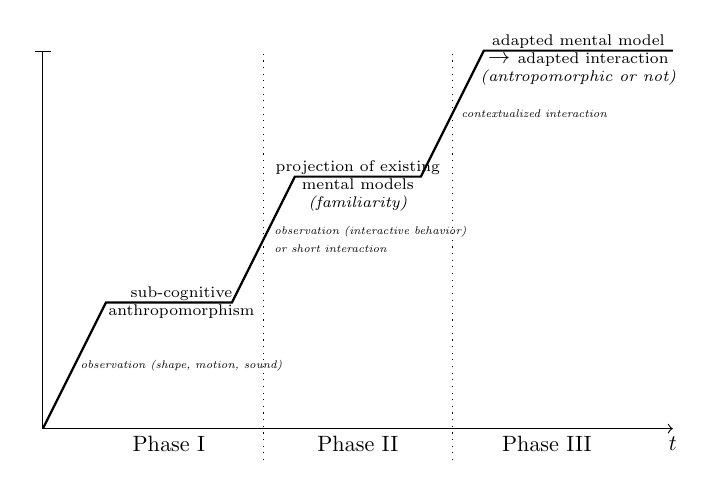
\begin{tikzpicture}[scale=0.8, transform shape]
\baselineskip=8pt

% horizontal axis
\draw[->] (0,0) -- (10,0) node[anchor=north] {$t$};
% labels
\draw   (2,0) node[anchor=north] {Phase I}
        (5,0) node[anchor=north] {Phase II}
        (8,0) node[anchor=north] {Phase III};

\draw[dotted] (3.5, -0.5) -- (3.5,6);
\draw[dotted] (6.5, -0.5) -- (6.5,6);

% vertical axis
\draw[-|] (0,0) -- (0,6) node[anchor=east] {};
% Us
\draw[thick] (0,0) -- (1,2) -- (3,2) -- (4,4) -- (6,4) -- (7,6) -- (10,6);

\draw (2.2,2) node[align=center] {\scriptsize{sub-cognitive}\\\scriptsize{anthropomorphism}}; %label
\draw (5,3.85) node[align=center] {\scriptsize{projection of existing}\\\scriptsize{mental models}\\\scriptsize{\it (familiarity)}}; %label
\draw (8.5,5.85) node[align=center] {\scriptsize{adapted mental model} \\ $\to$ \scriptsize{adapted interaction}\\\scriptsize{\it (antropomorphic or not)}}; %label

\draw (2.2,1) node[align=left] {\tiny{\it observation (shape, motion, sound)}}; %label
\draw (5.2,3) node[align=left] {\tiny \it observation (interactive behavior) \\ \tiny \it or short interaction}; %label
\draw (7.8,5) node[align=left] {\tiny \it contextualized interaction}; %label

\end{tikzpicture}
%}
\caption{The three cognitive phases of anthropomorphism: Phase I is the instinctive,
sub-cognitive identification of living peers. {\it Empathy} is characteristic
of this stage. After longer observation or short, uncontextualized interaction
(typically, a lab environment), the user enters Phase II: the user projects a
mental model he/she is already familiar with onto the robot. After longer {\it
contextualized} interaction (typically, at home), the user enters Phase III of
anthropomorphism: the user recomposes an accurate mental model of the robot,
based on experience. This leads to adapted interaction modalities, that may
still be anthropomorphic, or not.}
\label{fig:cognitivemodel}
\end{figure}

\paragraph{Building cognitive models over time}

Building on these previous researches, Figure~\ref{fig:cognitivemodel} offers a
cognitive perspective on the dynamics of anthropomorphism presented in the
previous section.

The first cognitive phase we identify that contribute to anthropomorphism is
actually \emph{pre-cognitive}. This is supported by studies like Rosenthal-von
der Pütten \textit{et al.}~\cite{rosenthal-vonderputten_experimental_2013} that
investigated the neural correlates of emotional reactions of human towards
robot.

After a longer observation period (typically including complete action
sequences of the robot) or short interaction (touching, short talk like
greetings), we suggest the human enters the cognitive \emph{phase II}: in this
phase, the human starts to build a behavioral and cognitive model of the robot
that would support both the observed and imagined capabilities of the robot.
The \emph{familiarity thesis}\fxfatal{citation!} would support the idea that
the human first projects onto the robot mental models of similar agents he/she
is already familiar with. This may range from animals to human adults, through
pets and children. We hypothesize that the nature of the projected mental
model, as well as how deep the human engages in this projection, might be
driven by the same parameters as we presented for the \emph{initial capital of
anthropomorphism} (section~\ref{sec:ica}).

We identify a further transition to the cognitive \emph{phase III} after a
\emph{contextualized} interaction. A \emph{contextualized} interaction is
\emph{explicitly purposeful} (the purpose of the interaction, be it purely
entertainment, is explicit and conscious for the human), and takes place in an
environment that fosters a stronger cognitive (and possibly affective)
commitment from the human in the interaction (typically, at home). During this
interaction, the human iteratively restate and reshape its behavioral and
mental model of the robot (\emph{How does the robot react to such and such
situation/input? What does the robot know about me? About itself? About our
environment? What can the robot learn?}, etc.).

This mental process heavily depends on the human understanding of the robot's
inner working, as well as his/her own tendency to anthropomorphize (the
\emph{personality} in ICA factor), but at this stage, the \emph{perception} of
the robot (its shape for instance) and its intended \emph{purpose} play a less
important role. It is mostly a human-centric process.

The result of this third phase is an iteratively adapted cognitive model of the
robot.

\paragraph{Relation to the model of anthropomorphism} It must be noted that the
three cognitive phases we introduce here do not match the
\emph{initialization}, \emph{familiarization} and \emph{stabilization} phases
introduced at~\ref{sec:phases}: in particular, cognitive phases I and II are
both included in the \emph{initialization} phase of the anthropomorphism model.

Sub-cognitive anthropomorphism typically \emph{initiates} the novelty effect by
rapidly engaging the human in the interaction through an initial projected
\emph{agency}, whereas cognitive phase II (projection of familiar mental
models) supports the novelty effect by inducing beliefs that the robot is set
up with possibly complex cognitive abilities.

The cognitive phase II also overlaps with the \emph{familiarization} phase: as
(s)he get used to the robot, we hypothesize the human restates and adapts its
cognitive model of the robot by iteratively reshaping pre-existent, familiar
models until it provides a satisfying support to explain and justify the
observed robot behavior.

A \emph{stable level of anthropomorphism} is reached when the adaptation
process depicted in cognitive phase III reached a stable state, \ie the human
experience with the robot is correctly supported by the cognitive model the
human has built.

\paragraph{Limits} This discussion on the cognitive correlates of the dynamics
of anthropomorphism are speculative, and only indirectly supported by
experimental evidence. New experiences need to be designed to specifically test
these hypothesis.\fxnote{...}

\section{Discussion}
\label{sec:discussion}

The model of anthropomorphism we propose is still a work in progress. In
particular, its exact implications regarding the design of (social) robots and
human-robot interaction are still to be investigated.

%\subsection{Effect of Context of Use and Purpose of the Robot}
%\label{sec:8.1}
%Frederic: role of uselessness
%
%
%\begin{description}
%
%    \item[\textbf{Hypothesis 1}] A person's tendency to anthropomorphize a
%        robot is impacted by the context of use and purpose of the robot. A
%        social context and purpose of the robot increases anthropomorphism.
%        \textit{(context and purpose of the robot)}
%
%\end{description}
%


\subsection{Effect of Time and Familiarization}
\label{sec:8.2}

The \textit{context of use} is related to the purpose (and functionality) of
the robot and influences the user interaction experience. With \textit{time},
we refer to long-term interaction with the robot, which is related to what has
been described as \textit{novelty effect} but also accounts for the user
getting used to the robot. Consequently, we propose that anthropomorphism is
not static but likely to change, due to what we call \textit{dynamics}, in
space and time.


As outlined in section \fixme{XX}, the tendency to anthropomorphize is
motivated by a person's wish to make sense of an agent which might be difficult
to understand (in its functionality or behavior, for instance). In turn, a user
might ascribe intentions or emotions to the system because the systems output
was unexpected for the user. Based on this explanation, we estimate that when
the user has familiarized herself / himself with the system, thus reached the
point of when the system is usable and explainable, the tendency to
anthropomorphize decreases. Therefore, our second hypothesis is as follows: 

\begin{description}

    \item[\textbf{Hypothesis 2}] A person's tendency to anthropomorphize a
        robot decreases over time and with growing experience the person has
        with the robot. \textit{(familiarize oneself with the robot)}

\end{description}	
	

Given our first hypothesis from above, this might not hold over all contexts;
more concretely, probably not in a social context of usage.


Smart innovative devices, such as personal domestic robots, might demand from a
human user spontaneous usage of an unfamiliar system. Such situations will
require that a user should be able to build up a mental model quickly, which
particularly holds for novice users \cite{schmitz_concepts_2011}.

Eddy \textit{et al.} points out that familiarity increases the tendency to
anthropomorphize \cite{eddy_attribution_1993}.

"As shown in several psychological experiments [13,24] and pointed out by Watt
[25], familiarity may also ease social acceptance and even tend to increase
people's tendency to anthropomorphize [16]." \cite{duffy_anthropomorphism_2003}

%\subsection{Personal characteristic effects in anthropomorphizing}
%\label{sec:8.3}

\subsection{Segmentation of interaction phases}

TBD

\subsection{Behavioral cues of anthropomorphism}
\label{sec:behavioralcues}

Our model suggests to analyze anthropomorphism based on a \emph{relative and
normalized level of anthropomorphic effects} instead of an absolute
quantitative assessment of anthropomorphic evidences. Similarly we introduce
two specific \emph{abstract} levels of anthropomorphism, the \emph{Initial
Capital of Anthropomorphism} and the \emph{Stabilized Level of
Anthropomorphism}: while we discuss the factors on which those values are
build, we did not formally investigated the experimental cues or evidences
that would allow to actually quantify those levels.

This is explained by the intricacy and interdependency of those behaviors.
Their correct identification and interpretation rely on psychosomatic cues that
the authors did not investigate.

A formal methodology for the assessment of anthropomorphic effects in HRI, as
well as a typology of these effects is still to be devised.


\section{Conclusion}
\label{sec:9}

\fxfatal{To be extended}

Anthropomorphism is a social phenomenon, which seems to be natural on one side
and very complex on the other side. It is a mechanism within oneself that makes
a human observer think and treat a non-human agent as if it would have some
human (social) characteristics, and ascribe to it intentions, emotions, or
thoughts, for instance. In accordance with other researchers, we also think
that the term is sometimes misused or misunderstood
\cite{duffy_anthropomorphism_2002}. Concerning robotics, we do not think that
we can speak of anthropomorphism when a person simply refers to physical parts
of a robot using terms that describe a human body, such as arm, head, fingers,
etc.. We believe that this is not anthropomorphism in its true sense because
the person might simply take advantage of the physically resembling shape
instead of truly ascribing human (social) characteristics to the robot.



\section*{Acknowledgements}
AJung Moon, Aude Billard.\\

This research was supported by the Swiss National Science Foundation through
the National Centre of Competence in Research Robotics.


\bibliographystyle{abbrv}
\bibliography{biblio} 
%Generated by bibtex from your ~.bib file.  Run latex,
%then bibtex, then latex twice (to resolve references)
%to create the ~.bbl file.  Insert that ~.bbl file into
%the .tex source file and comment out
%the command \texttt{{\char'134}thebibliography}.
\balancecolumns
\end{document}
